\section{Intro}
\begin{frame}{What}
	\begin{block}{library}
		\begin{itemize}
			\item Intended to be used by client plugin
			\item LGPLv3+
			\item Written in around 2300 lines of C
			\item Only depends on libgcrypt 1.6+
			\item Standard crypto stuff adapted from GNUnet
		\end{itemize}
	\end{block}
\end{frame}

\begin{frame}{library design}
	\begin{figure}
		\centering
		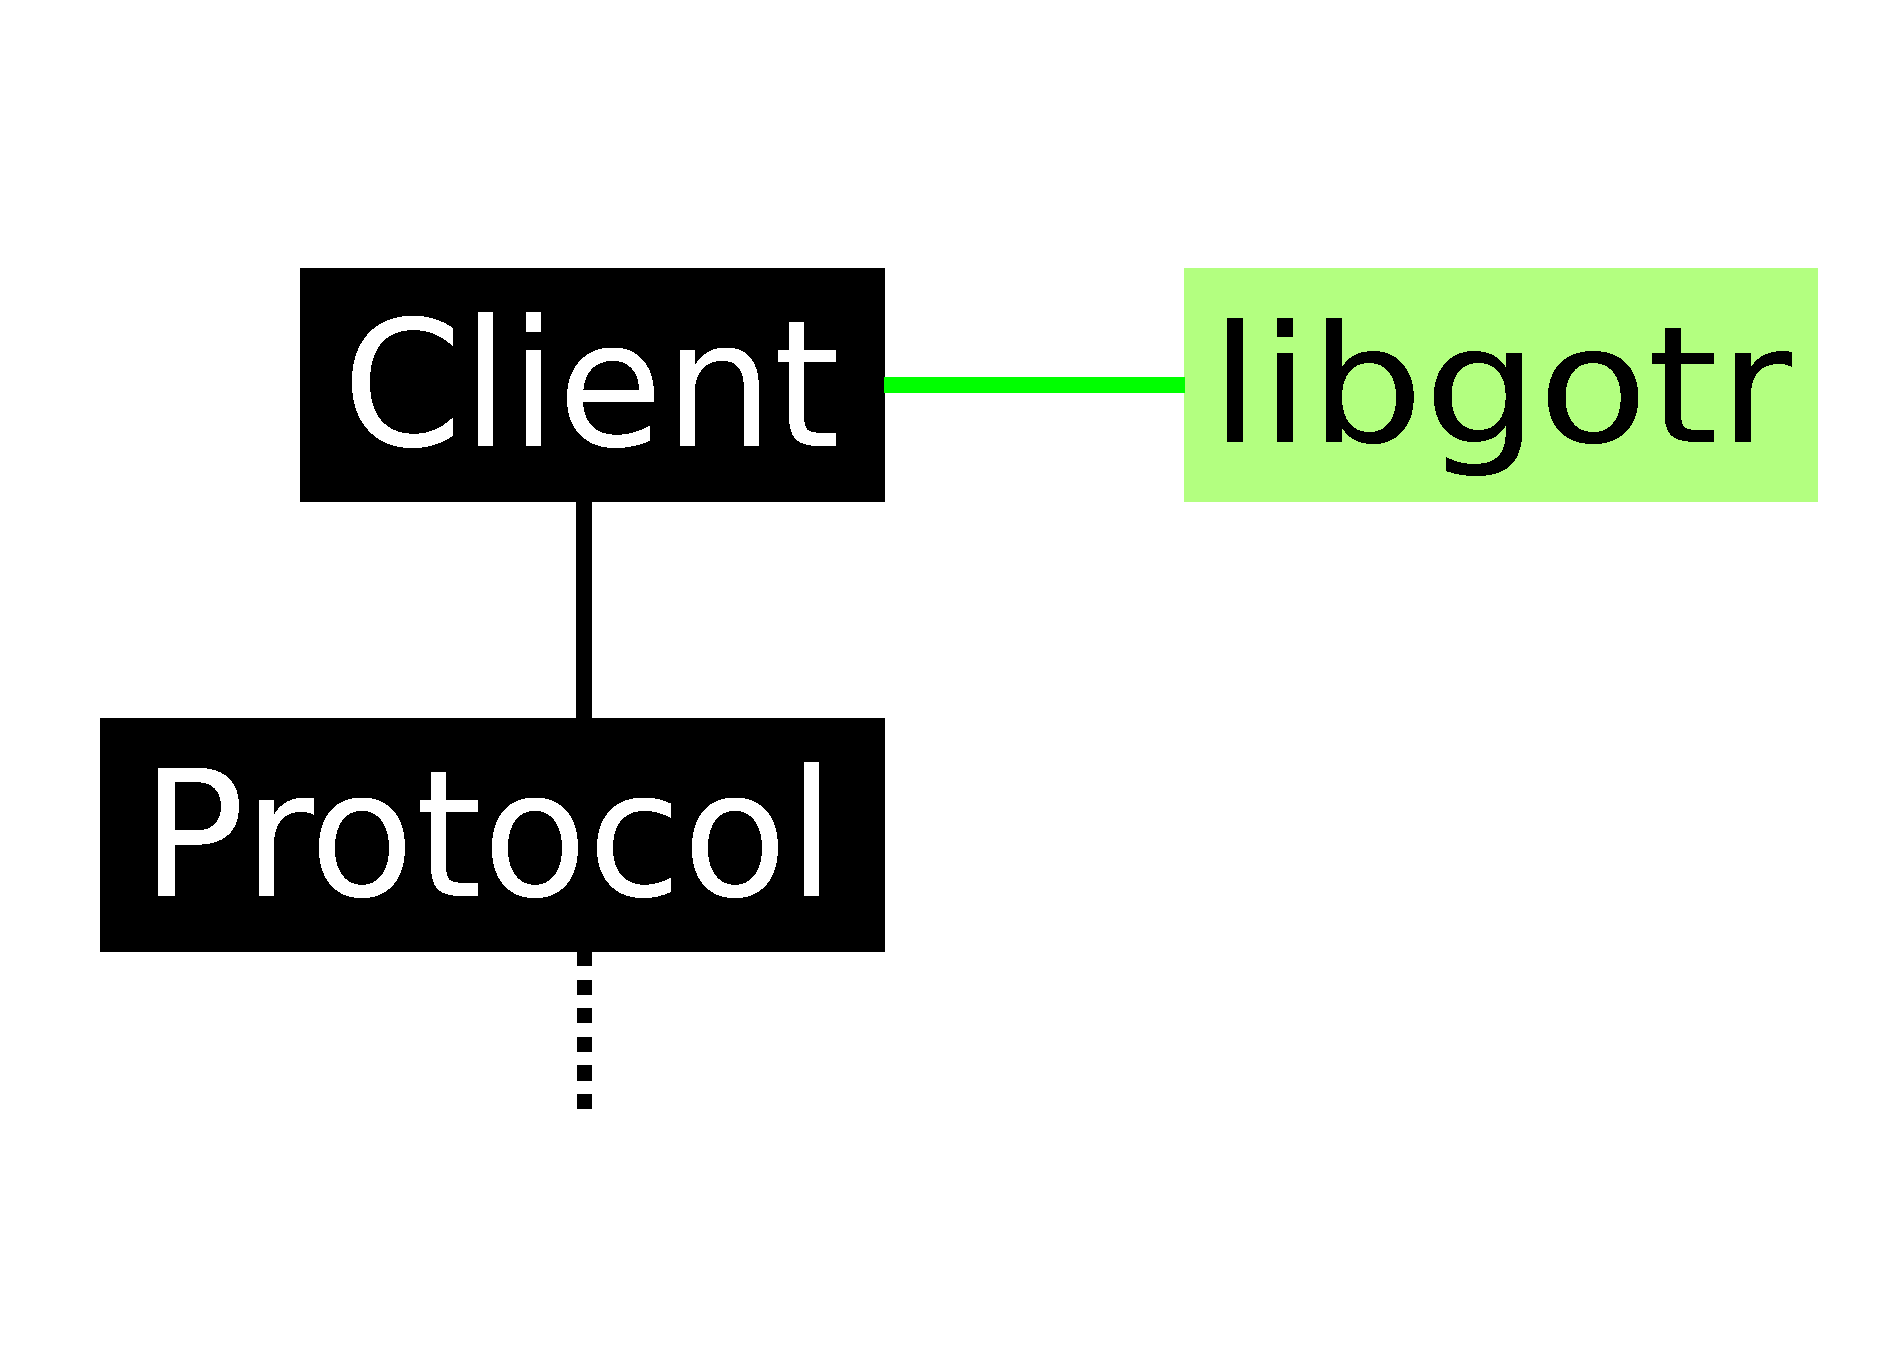
\includegraphics[width = 0.9\textwidth]{./abbildungen/arch_client.eps}
	\end{figure}
\end{frame}

\begin{frame}{Introduction}
	\begin{alertblock}{Disclaimer}
		\begin{itemize}
			\item No real crypto auditing yet
			\item Not yet checked for thread safety
			\item Only tested on GNU/Linux and Mac OS X
		\end{itemize}
	\end{alertblock}
\end{frame}

\begin{frame}{Goal}
	\begin{block}{We try to achieve the following properties}
		\begin{itemize}
			\item Authenticity
			\item Integrity
			\item Confidentiality
			\item Deniability
			\item Forward Secrecy
			\item Consensus
		\end{itemize}
	\end{block}
\end{frame}

\begin{frame}{Assumptions}
	\begin{block}{For libgotr to be usable we assume}
		\begin{itemize}
			\item Underlay protocol manages IDs and rooms
			\item (Un)limited message length
			\item Reliable, in-order packet transmission
			\item Low latency
			\item Some more bandwidth for crypto overhead
		\end{itemize}
	\end{block}
\end{frame}
